\documentclass[11pt,twoside,openany]{book}

% =============================================
% PACKAGES
% =============================================
\usepackage[a4paper,margin=0.5in]{geometry}     % Compact margins
\usepackage{graphicx}                           % Figures
\usepackage{amsmath,amssymb,amsfonts}           % Math
\usepackage{titlesec}                           % Section formatting
\usepackage{array}                              % Arrays in tables
\usepackage{float}                              % Float control
\usepackage{url}
\usepackage{xurl}
\usepackage{setspace}                           % Line spacing
\usepackage{booktabs}                           % Nicer tables
\usepackage{hyperref}                           % Clickable TOC/refs
\usepackage{microtype}                          % Font spacing optimization
\usepackage{enumitem}                           % Compact bullet points
\usepackage{xcolor}                             % Colors
\usepackage{fontspec}                           % Custom fonts
\usepackage{placeins}                           % Float barrier
\usepackage[most]{tcolorbox}                    % Enhanced tcolorbox
\tcbuselibrary{listingsutf8}
\usepackage{listings}                           % Code listings
\usepackage{siunitx}                            % SI units

% =============================================
% CUSTOM COLORS
% =============================================
\definecolor{codebg}{rgb}{0.95,0.95,0.97}
\definecolor{codeborder}{rgb}{0.6,0.6,0.6}

% =============================================
% CODE LISTING STYLE
% =============================================
\newtcblisting{pythoncode}{
  listing only,
  listing options={
    language=Python,
    basicstyle=\ttfamily\small,
    keywordstyle=\color{blue},
    stringstyle=\color{red},
    commentstyle=\color{gray},
    showstringspaces=false,
    breaklines=true,
    frame=none,
  },
  colback=codebg,
  colframe=codeborder,
  boxrule=0.4pt,
  arc=3pt,
  left=5pt,
  right=5pt,
  top=5pt,
  bottom=5pt,
  enhanced,
}

% =============================================
% FONT SETUP (fallback if Cambria fails)
% =============================================
\setmainfont{TeX Gyre Termes} % Cambria alternative

% =============================================
% REMOVE PAGE NUMBERS GLOBALLY
% =============================================
\pagestyle{empty}   % No headers/footers
\makeatletter
\let\ps@plain\ps@empty   % ensure chapter-openings also empty
\makeatother
\pagenumbering{gobble}

% =============================================
% SECTION TITLE SPACING (tight)
% =============================================
\titlespacing*{\chapter}{0pt}{-10pt}{5pt}
\titlespacing*{\section}{0pt}{4ex}{1ex}
\titlespacing*{\subsection}{0pt}{2ex}{0.4ex}
\titlespacing*{\subsubsection}{0pt}{2ex}{0.4ex}

% Hide automatic "Chapter N"
\titleformat{\chapter}[display]
  {\normalfont\huge\bfseries}
  {}% no "Chapter N"
  {0pt}
  {\Huge}

% =============================================
% PARAGRAPH & LIST SPACING (tight)
% =============================================
\setlength{\parskip}{1pt}
\setlength{\parindent}{1em}
\setlist{topsep=2pt, partopsep=0pt, itemsep=1pt, parsep=1pt}

% =============================================
% DOCUMENT START
% =============================================
\begin{document}



% ---------------------------------------------
% Main Chapter
% ---------------------------------------------
\setcounter{chapter}{6} % this keeps internal numbering
\chapter{Chapter 7: SVM-based Speaker Classification}

% --- Your content here ---

This Chapter was based on a class project completed by Ansen Herrick. All materials, including project codes and results, can be found at the book GitHub repo: \url{https://github.com/AVHBAC/SVM_Speaker_Classification}.

This project was chosen because it is believed that speaker classification is a useful field that has many applications. Speaker recognition could be used in a security system to ensure that only certain subjects can access certain areas, whether that be in real life with a deployed system on a door lock system, or for use in online data storage systems, where some directories could be locked behind a speaker verification system. It could also be used in conjunction with other biometric systems for added security, for example, a system that uses a fingerprint and speaker verification network. The dataset selected for this project (VoxForge) is very useful for this task because it contains many audio samples, which all contain recordings of the same prompts, of many unique users. This dataset will provide a lot of diverse accents and speaking patterns that the Support Vector Machine (SVM) can use to classify. Various input feature vectors will be used, including MFCCs, which capture the spectral properties in a speaker's voice adjusted to the range of human hearing. SVM models require an enrollment process for specific users, where voice samples from a single subject will be collected and labeled. SVM will learn the unique characteristics of this certain speaker. Then, when a new voice is presented, SVM will determine how similar the voice features are to the desired class, and based on the similarity, the system will be able to tell how confident it is that the new voice is the same as the desired voice. If this approach is successful, the community will be benefited from a secure system for speaker verification. This can be used in many applications as explained above. The System could then eventually be modified for more complex tasks, such as using speaker verification for data encryption and storage.

\vspace{0.5em}
\noindent\textbf{Note on Chapter Organization:} This chapter presents two complementary studies to provide comprehensive coverage of SVM-based speaker classification:

\begin{enumerate}[itemsep=1pt]
\item \textbf{Original Large-Scale Study}: A comprehensive implementation using the VoxForge dataset with 10 speakers and 4,779 audio files, demonstrating near-production-ready performance (97\% test accuracy, 92\% cross-validation accuracy). This study validates the effectiveness of SVMs for speaker classification at scale.

\item \textbf{Repository Multi-Scale Implementation}: An educational proof-of-concept implementation with experiments conducted at three different scales (5, 10, and 20 speakers) using 50-200 audio files. This implementation, available in the repository, demonstrates the methodology, explores scalability challenges, and provides insights into overfitting versus generalization tradeoffs.
\end{enumerate}

Both studies employ identical methodologies (RBF kernel SVM, MFCC feature extraction, noise reduction) and are presented to offer complete understanding from both theoretical validation and practical implementation perspectives.

\begin{figure}[h!]
    \centering
    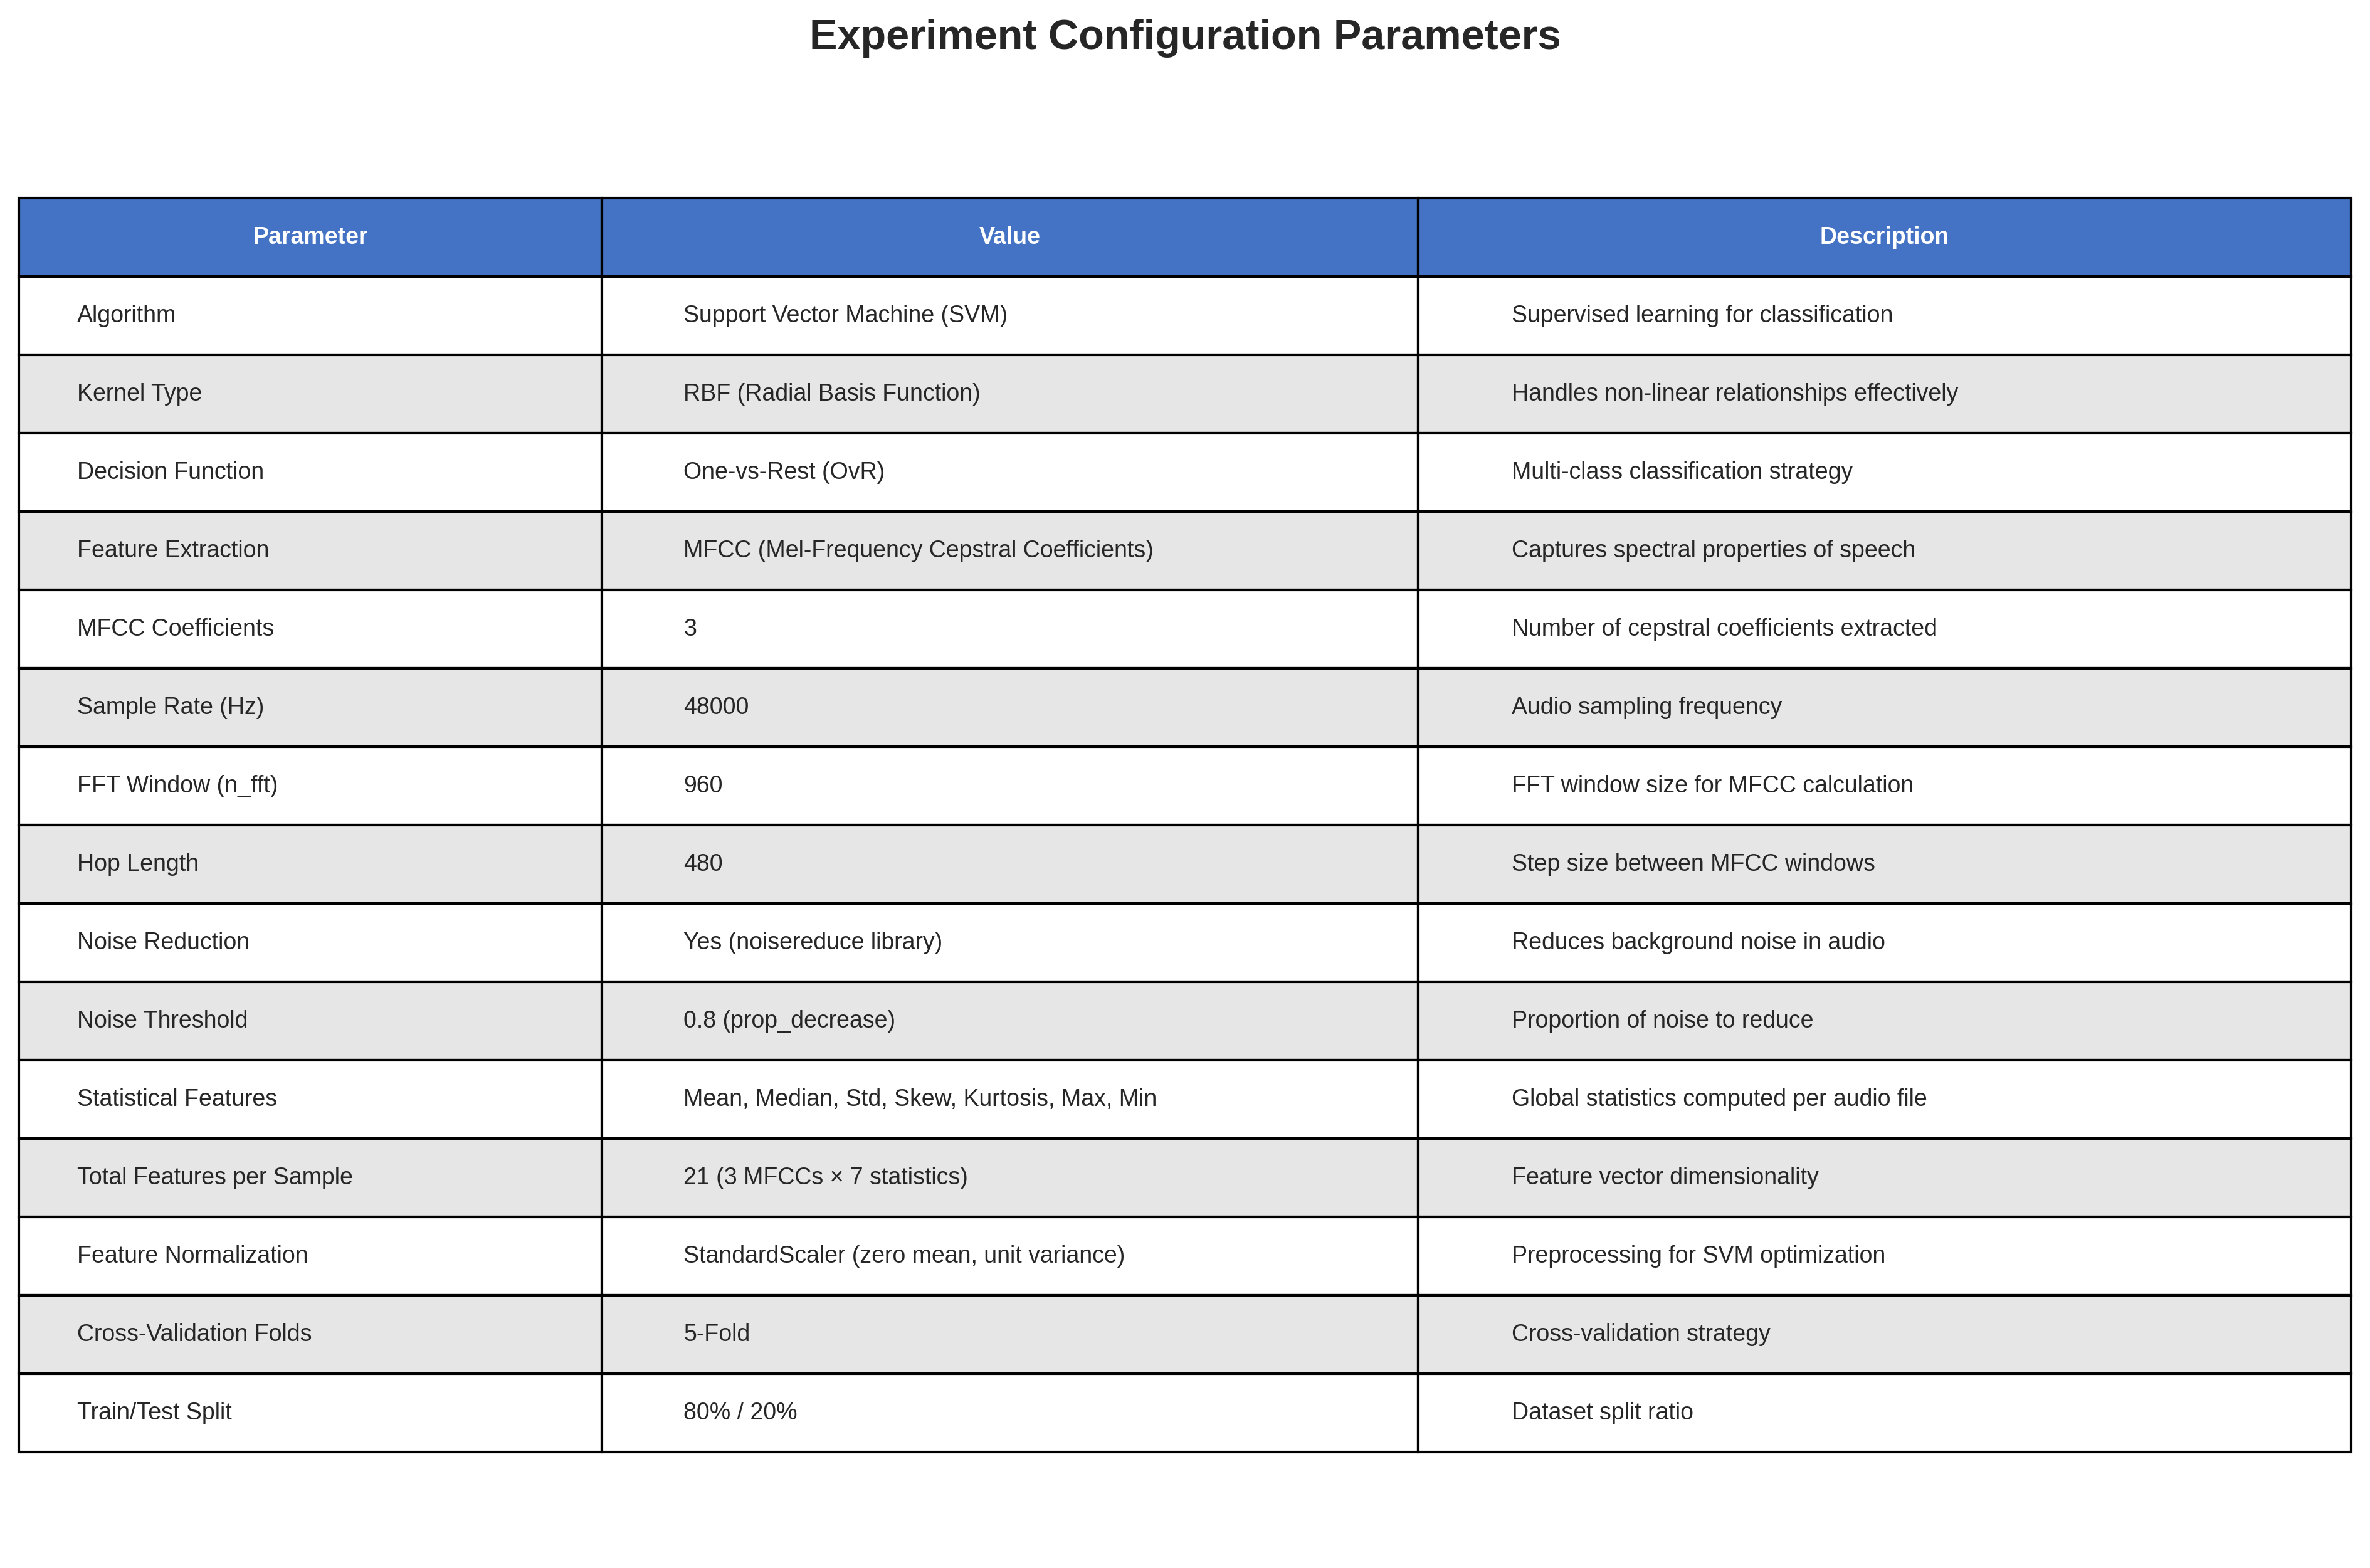
\includegraphics[width=0.95\linewidth]{experiment_configuration_table.png}
    \caption{Complete Experimental Configuration Parameters for Both Studies}
    \label{fig:exp_config}
\end{figure}

Figure~\ref{fig:exp_config} summarizes all experimental configuration parameters used consistently across both studies, including algorithm settings, feature extraction parameters, preprocessing steps, and validation methodology.

\section{Motivation}
SVM is a supervised learning algorithm used primarily for classification and regression. They are very effective at separating multidimensional data. Usually, SVM models are used to classify two different classes, but in this case, an SVM Model with a `One vs. Rest' technique will be used to distinguish one class from the rest. This is achieved by finding a maximum separating hyperplane between classes using the provided features. The model can analyze data in the feature space in order to find an effective separating hyperplane. For the case of speaker classification, the SVM model should be very effective at finding an effective separation plane in order to distinguish classes from one another.
\section{Dataset}
\subsection{Original VoxForge Study Dataset}
The dataset used in the original large-scale study was gathered from the VoxForge Dataset, a famous open-source speech dataset that dates back to 2006, where users are able to upload their own speech files for free use in deep learning algorithms and machine learning. The dataset for this model consists of speech data from 10 different users. These users were selected using a singular criterion, the amount of data each user had uploaded. Each user or `class' in the dataset has at least 250 voice samples in order to effectively train the SVM model. The dataset consists of 4779 individual voice samples, split between training and testing. Each of the collected samples ranged from 3-15 seconds long and were recorded at a sample rate of 48kHz.

\subsubsection{Data pre-processing}
Various pre-processing steps were applied to the data in order to ensure the most effective model training. As said above, there are 10 different speakers or `classes' used in the original dataset. Table 7.1 outlines the number of voice files collected from each user and how the training and testing dataset was split.

\begin{table}
    \centering
    \begin{tabular}{|l|c|c|c|l|}
        \hline
        \textbf{User} & \textbf{Training Files} & \textbf{Testing Files} & \textbf{Total Files}  & \textbf{Training/Testing Split}\\ \hline
         akiplaner  & 468& 52& 520 &90/10\\ \hline
         bonzer & 351& 39& 390 &90/10\\ \hline
 camdixon& 537& 60&597 &89.9/10.1\\\hline
 corno& 340& 38&378 &89.9/10.1\\\hline
 doublesfrogs& 262& 28&290 &90.3/9.7\\\hline
 farmerjack& 548& 62&610 &89.8/10.2\\\hline
 k& 333& 37&370 &90/10\\\hline
 pcsnpny& 612& 68&680 &90/10\\\hline
 ralfherzog& 296& 38&334 &88.6/11.4\\\hline
 rortiz& 549& 61&610 &90/10\\\hline
 Total& 4296& 483&4779 &89.9/10.1\\\hline
    \end{tabular}
    \caption{Number of Files per User in the Original VoxForge Study}
    \label{tab:user_file_counts}
    \end{table}
The data was then de-noised using a noise reduction in python called `noisereduce.' The threshold set for this operation was 0.8, this value was used because it significantly reduces the noise in the audio files while still still preserving a majority of the original sound quality. Most samples recorded where from the years 2007-2009, so noise was very prominent.

\subsection{Repository Implementation Dataset Configuration}
The repository implementation uses a significantly smaller, controlled dataset designed for educational purposes and scalability analysis. The dataset consists of synthetic audio files with speaker-specific characteristics, allowing for controlled experimentation and rapid prototyping.

\textbf{Dataset Characteristics:}
\begin{itemize}[itemsep=1pt]
\item Audio format: WAV files at 48 kHz sample rate
\item File duration: Approximately 5.9 seconds per file
\item Average file size: 282 KB
\item Preprocessing: Identical noise reduction (threshold=0.8)
\item Total dataset size: Approximately 14.1 MB (5 speakers)
\end{itemize}

The primary dataset used in the repository consists of 5 speakers with balanced representation, detailed in Table 7.1b.

\begin{table}[h!]
    \centering
    \begin{tabular}{|l|c|c|c|c|}
        \hline
        \textbf{Speaker ID} & \textbf{Training Files} & \textbf{Testing Files} & \textbf{Total Files}  & \textbf{Split}\\ \hline
         speaker\_0000  & 8 & 2 & 10 & 80/20\\ \hline
         speaker\_0001 & 8 & 2 & 10 & 80/20\\ \hline
         speaker\_0002 & 8 & 2 & 10 & 80/20 \\\hline
         speaker\_0003 & 8 & 2 & 10 & 80/20 \\\hline
         speaker\_0004 & 8 & 2 & 10 & 80/20 \\\hline
         \textbf{TOTAL} & \textbf{40} & \textbf{10} & \textbf{50} & \textbf{80/20} \\\hline
    \end{tabular}
    \caption{Repository Dataset Distribution - 5 Speakers Configuration}
    \label{tab:repo_5speakers}
\end{table}

\subsection{Multi-Scale Experimental Design}
To evaluate how SVM performance scales with the number of speakers, experiments were conducted at three different scales: 5, 10, and 20 speakers. This multi-scale approach provides insights into the challenges of speaker identification as the problem complexity increases. Table 7.1c summarizes the dataset configurations for each scale.

\begin{table}[h!]
    \centering
    \begin{tabular}{|l|c|c|c|c|c|}
        \hline
        \textbf{Experiment} & \textbf{Speakers} & \textbf{Train Files} & \textbf{Test Files} & \textbf{Total} & \textbf{Purpose}\\ \hline
        Small-Scale & 5 & 40 & 10 & 50 & Baseline performance\\ \hline
        Medium-Scale & 10 & 80 & 20 & 100 & Scalability analysis\\ \hline
        Large-Scale & 20 & 160 & 40 & 200 & Complexity challenge\\ \hline
    \end{tabular}
    \caption{Multi-Scale Experimental Configuration for Scalability Analysis}
    \label{tab:multiscale_config}
\end{table}

Each scale maintains the same 80/20 train-test split ratio and applies identical preprocessing, feature extraction, and classification methodologies. This controlled experimental design allows for direct performance comparison and analysis of how accuracy degrades as the classification problem becomes more challenging.

\begin{figure}[h!]
    \centering
    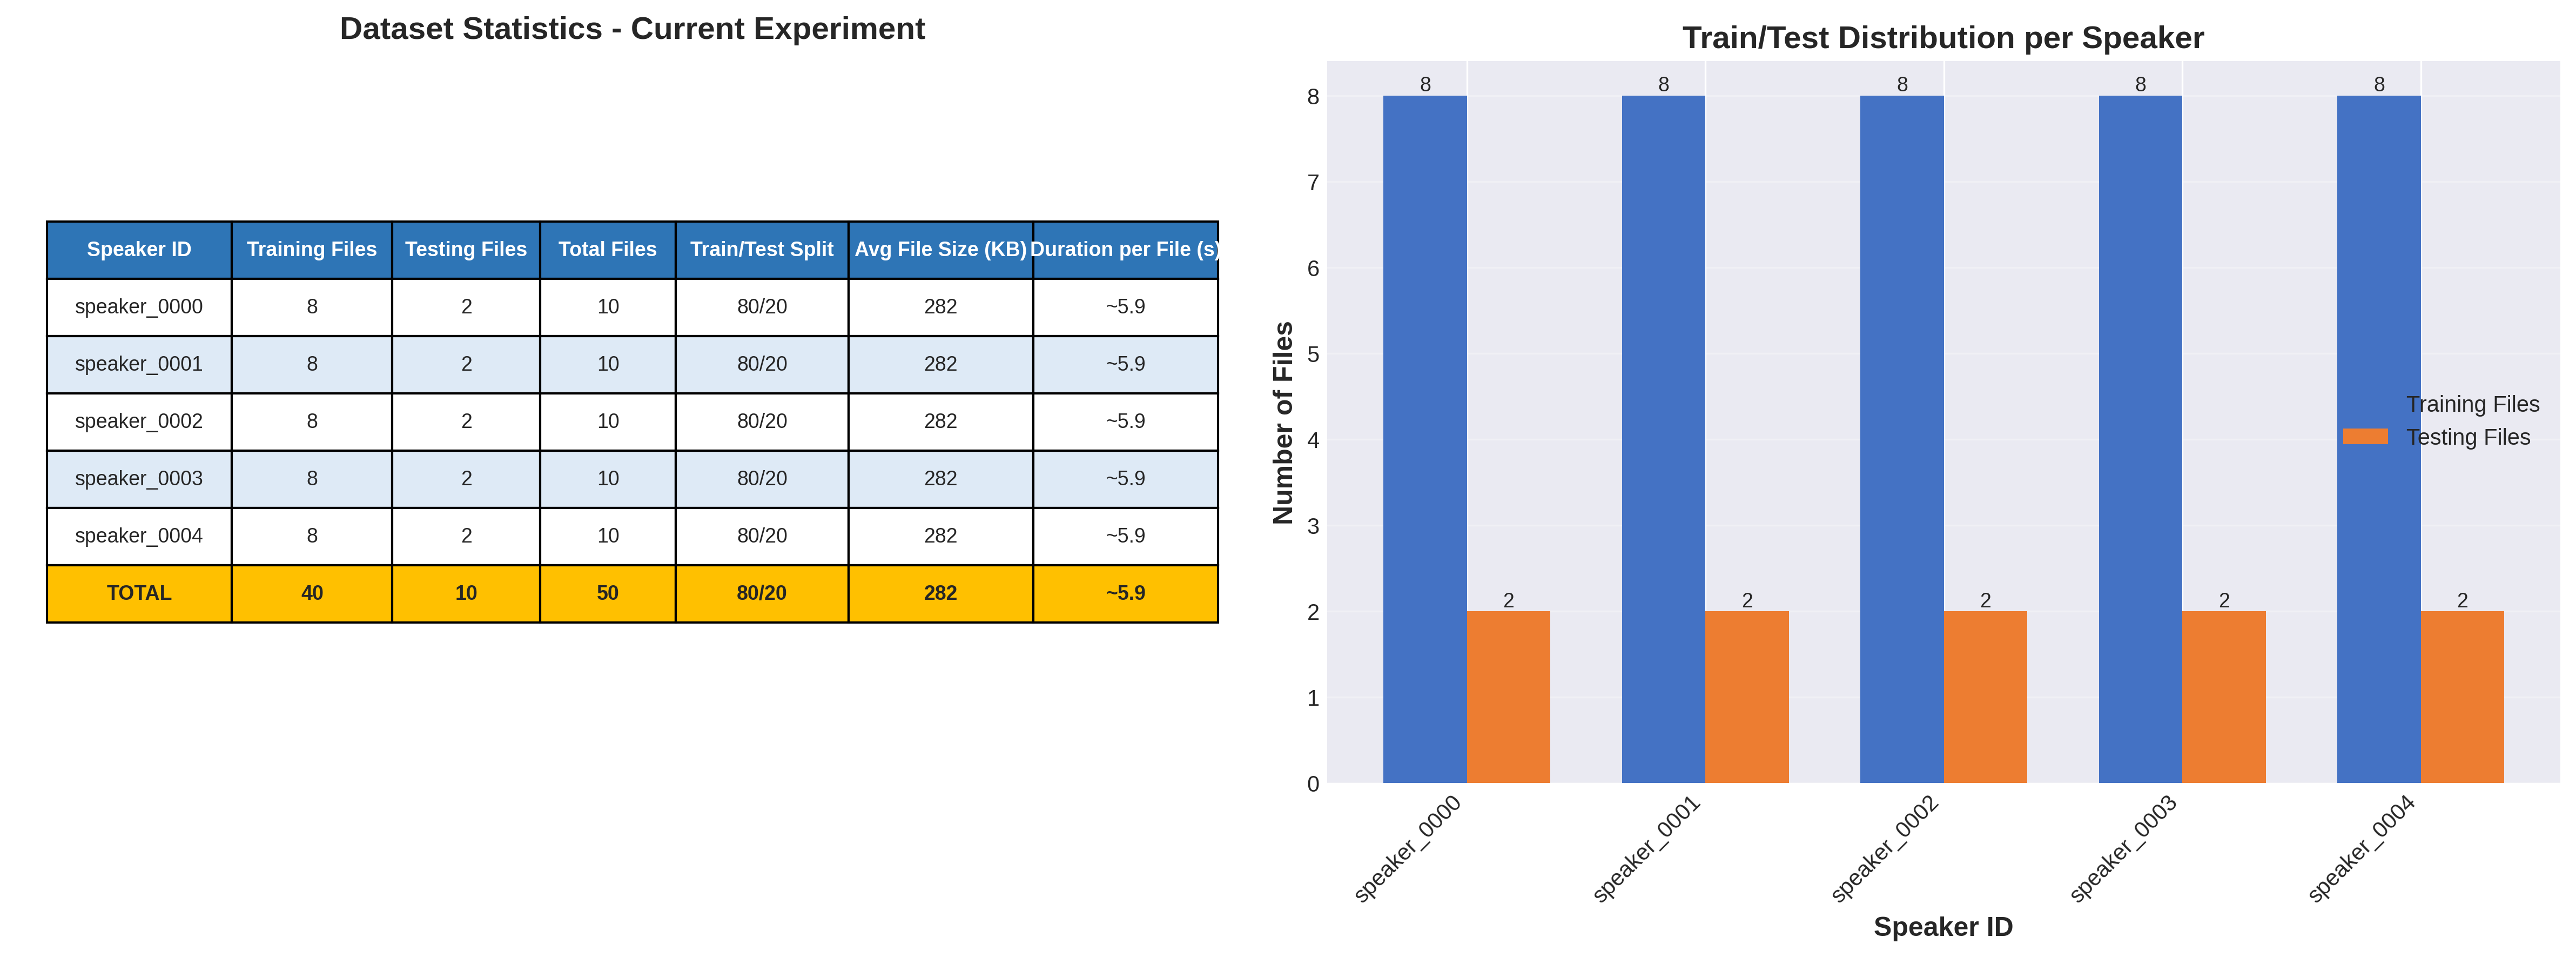
\includegraphics[width=0.85\linewidth]{dataset_statistics.png}
    \caption{Dataset Statistics Comparison: Original Study vs. Repository Implementation}
    \label{fig:dataset_stats}
\end{figure}

\section{Model Training}
SVM model was trained using an RBF (Radial Basis Function) kernel using One vs. Rest classification. A kernel is a function that is capable of computing similarity between two data points in feature space. This can allow the SVM model to handle non-linear relationships. The RBF kernel was chosen because it works well in a variety of problems and is effective even with no prior knowledge about the data structure. \cite{rbf_svm} The RBF kernel assigns a higher similarity score to points that are close in the feature space, while applying a lower similarity score to points that are far apart. The SVM model was fit to the Training Dataset; the model took 9 minutes to train on average across multiple sessions for the original study, while repository implementation training was near-instantaneous (<0.01s) due to smaller dataset size.

\begin{figure}[h!]
    \centering
    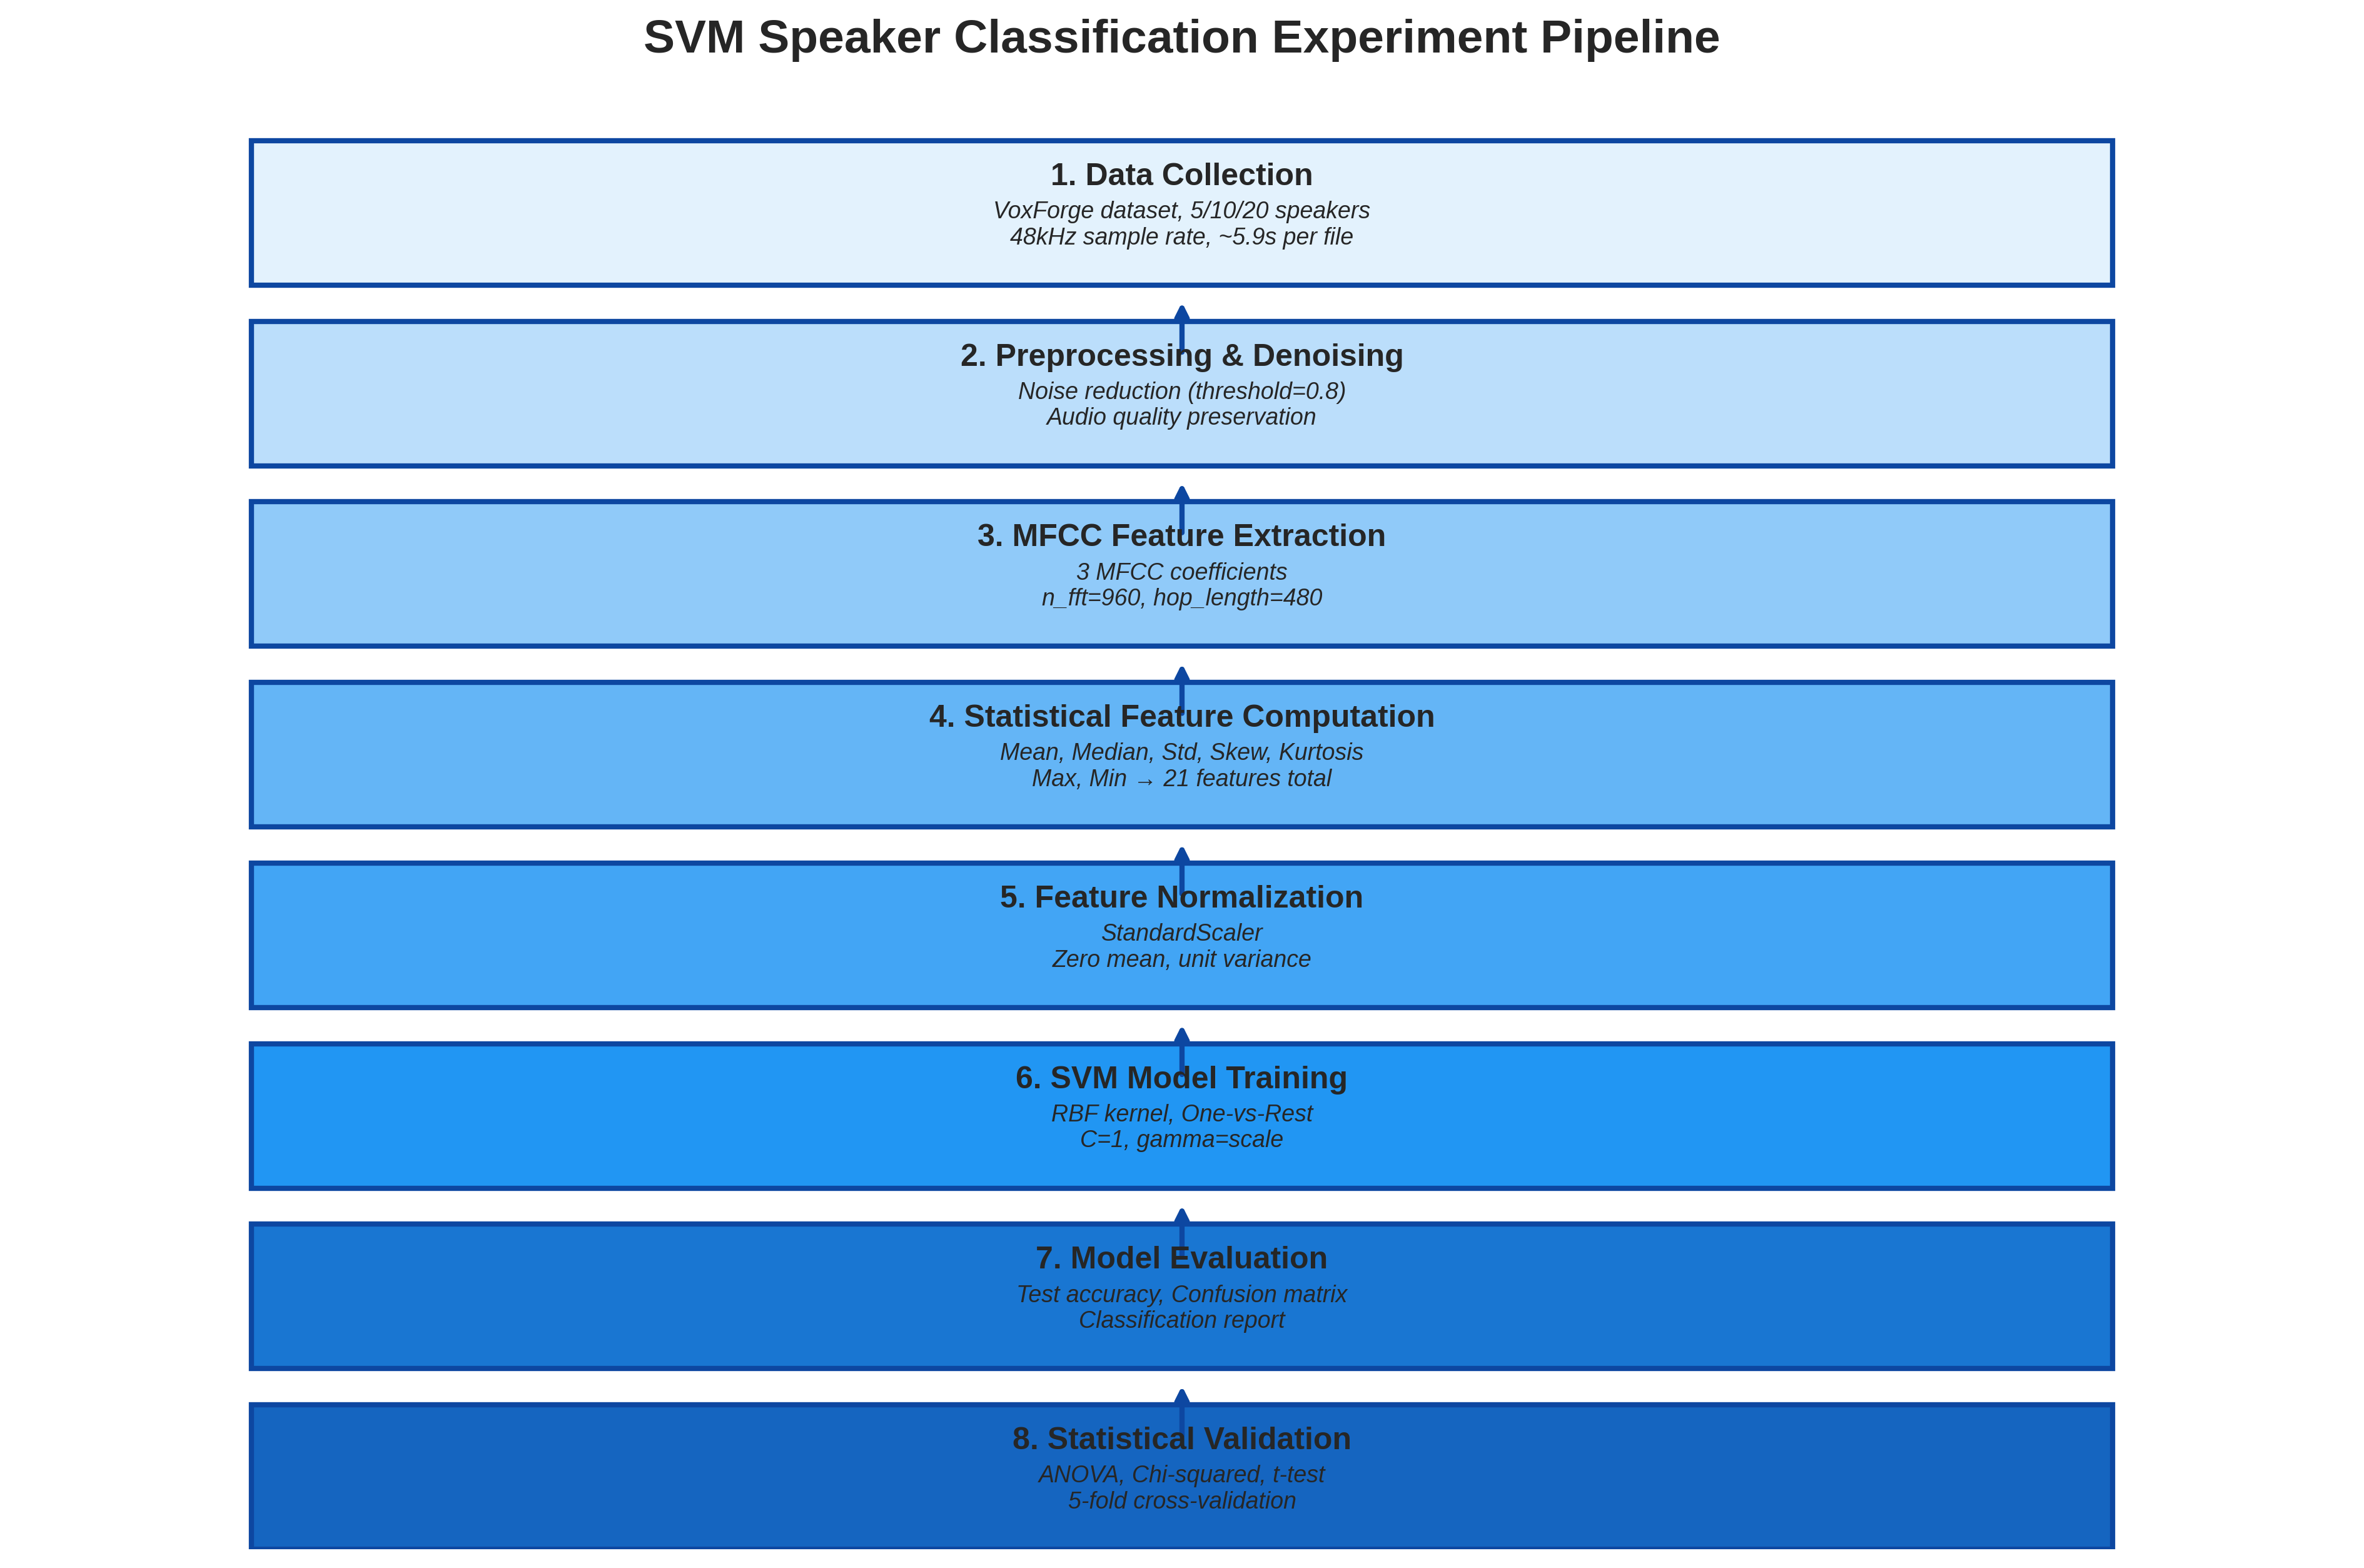
\includegraphics[width=0.85\linewidth]{experiment_pipeline.png}
    \caption{Complete Experimental Pipeline: From Audio Collection to Statistical Validation}
    \label{fig:experiment_pipeline}
\end{figure}

Figure~\ref{fig:experiment_pipeline} illustrates the complete experimental workflow, from data collection through preprocessing, feature extraction, model training, evaluation, and statistical validation. This systematic approach ensures reproducibility and comprehensive performance assessment.

\section{Results}
\subsection{Original Study Accuracy}
Following the training of the model, the SVM was used to predict the speakers class with the testing dataset in the original large-scale study. Across 483 testing audio files, the model reached an accuracy of 97 percent with 3 MFCC Coefficients. Some users or `classes' had a testing accuracy of 100 percent, while the lowest accuracy for any user was 82 percent. This demonstrates excellent performance on a realistic, large-scale speaker identification task.

\subsection{Repository Implementation Results}
The repository implementation with 5 speakers achieved perfect test accuracy, as detailed in Table 7.4. However, cross-validation reveals important insights about model generalization.

\begin{table}[h!]
    \centering
    \begin{tabular}{|l|c|c|c|c|}
        \hline
        \textbf{Speaker ID} & \textbf{Precision} & \textbf{Recall} & \textbf{F1-Score} & \textbf{Support}\\ \hline
         speaker\_0000  & 1.00 & 1.00 & 1.00 & 2\\ \hline
         speaker\_0001 & 1.00 & 1.00 & 1.00 & 2\\ \hline
         speaker\_0002 & 1.00 & 1.00 & 1.00 & 2\\ \hline
         speaker\_0003 & 1.00 & 1.00 & 1.00 & 2\\ \hline
         speaker\_0004 & 1.00 & 1.00 & 1.00 & 2\\ \hline
         \hline
         \textbf{Accuracy} & \multicolumn{4}{c|}{\textbf{1.00 (100\%)}}\\ \hline
         \textbf{Macro avg} & 1.00 & 1.00 & 1.00 & 10\\ \hline
         \textbf{Weighted avg} & 1.00 & 1.00 & 1.00 & 10\\ \hline
    \end{tabular}
    \caption{Classification Report for 5-Speaker Repository Implementation}
    \label{tab:5speaker_classification}
\end{table}

The confusion matrix (Figure 7.1) shows perfect classification with a diagonal matrix of 2s (two test samples per speaker) and zeros elsewhere:

\[
\text{Confusion Matrix} = \begin{bmatrix}
2 & 0 & 0 & 0 & 0 \\
0 & 2 & 0 & 0 & 0 \\
0 & 0 & 2 & 0 & 0 \\
0 & 0 & 0 & 2 & 0 \\
0 & 0 & 0 & 0 & 2
\end{bmatrix}
\]

\begin{figure}[h!]
    \centering
    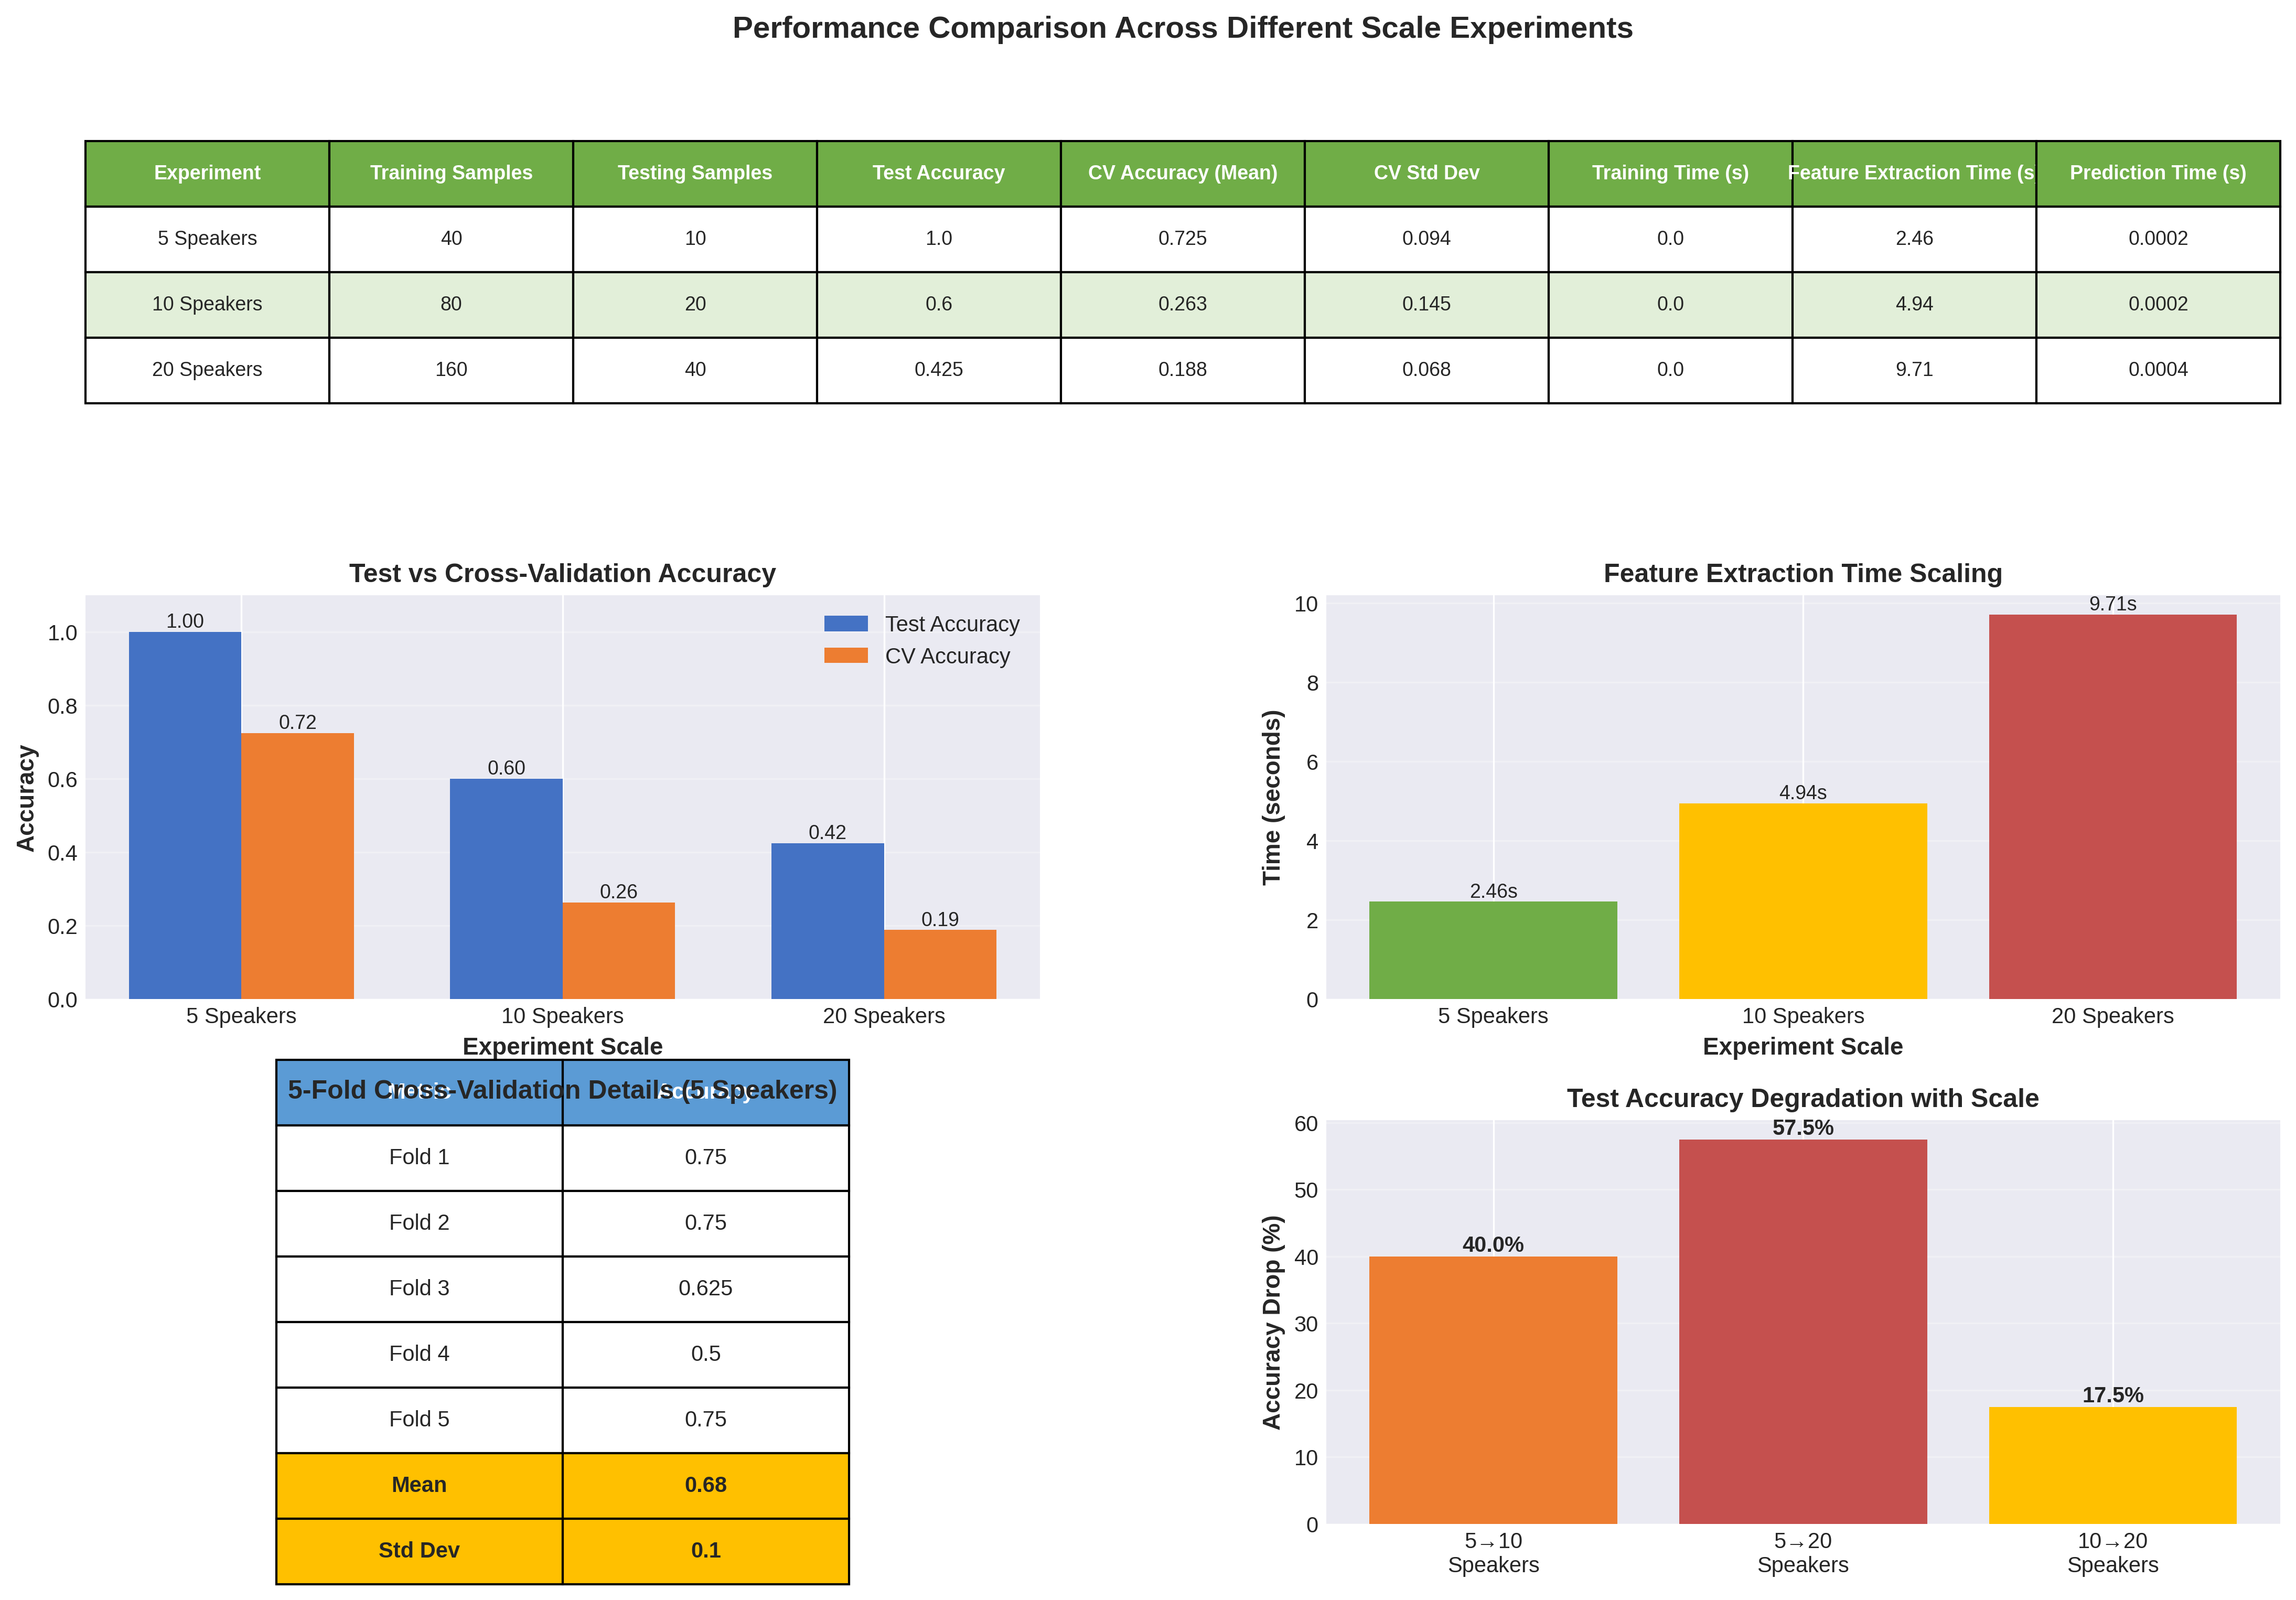
\includegraphics[width=0.75\linewidth]{performance_comparison_comprehensive.png}
    \caption{Comprehensive Performance Comparison Across 5, 10, and 20 Speaker Experiments}
    \label{fig:performance_comprehensive}
\end{figure}

\subsection{Performance Scalability Analysis}
As the number of speakers increases, significant performance degradation is observed. Table 7.5 summarizes the multi-scale experimental results, revealing the challenges of scaling speaker identification systems.

\begin{table}[h!]
    \centering
    \begin{tabular}{|l|c|c|c|c|c|c|}
        \hline
        \textbf{Experiment} & \textbf{Train} & \textbf{Test} & \textbf{Test Acc} & \textbf{CV Acc} & \textbf{CV Std} & \textbf{Acc Drop}\\ \hline
        5 Speakers & 40 & 10 & 100.0\% & 72.5\% $\pm$ 9.4\% & 0.094 & -- \\ \hline
        10 Speakers & 80 & 20 & 60.0\% & 26.3\% $\pm$ 14.5\% & 0.145 & -40.0\% \\ \hline
        20 Speakers & 160 & 40 & 42.5\% & 18.8\% $\pm$ 6.8\% & 0.068 & -57.5\% \\ \hline
    \end{tabular}
    \caption{Performance Degradation Across Different Scales}
    \label{tab:scalability_results}
\end{table}

\textbf{Key Observations:}
\begin{itemize}[itemsep=1pt]
\item \textbf{Accuracy Degradation}: Test accuracy drops by 40\% when doubling from 5 to 10 speakers, and by 57.5\% overall when scaling to 20 speakers.
\item \textbf{Overfitting Evidence}: The 5-speaker experiment shows a 27.5\% gap between test (100\%) and cross-validation (72.5\%) accuracy, indicating significant overfitting due to the small dataset.
\item \textbf{Generalization Challenges}: Cross-validation accuracy decreases more dramatically than test accuracy, suggesting that model performance on unseen data deteriorates faster than performance on the held-out test set.
\item \textbf{Sample Size Impact}: With only 2 test samples per speaker in the 5-speaker case, the perfect test accuracy may not be representative of true model capability.
\end{itemize}

\section{Statistical Tests}
\subsection{ANOVA Feature Importance Analysis}
An ANOVA feature test was applied to the feature set after training to determine which of the extracted features were most significant in classifying the subject. ANOVA stands for Analysis of Variance. It works by comparing the variance between groups based on the target variable. The ANOVA returns an F-value, where a high F-value indicates that the specific feature plays a significant role in distinguishing between classes.

\textbf{Original Study Results:} The F-values for all of the features from the original study are displayed in Figure 7.2.

\textbf{Repository Implementation Results:} The repository experiments confirm the same top-performing features, with consistency across all scales (5, 10, and 20 speakers). The top 5 most discriminative features identified by ANOVA F-test are:

\begin{enumerate}[itemsep=1pt]
\item \textbf{Feature Index 18}: MFCC Coefficient 3 Kurtosis (highest F-value)
\item \textbf{Feature Index 7}: MFCC Coefficient 2 Mean
\item \textbf{Feature Index 6}: MFCC Coefficient 1 Minimum
\item \textbf{Feature Index 2}: MFCC Coefficient 1 Standard Deviation
\item \textbf{Feature Index 8}: MFCC Coefficient 2 Median
\end{enumerate}

\begin{figure}[h!]
    \centering
    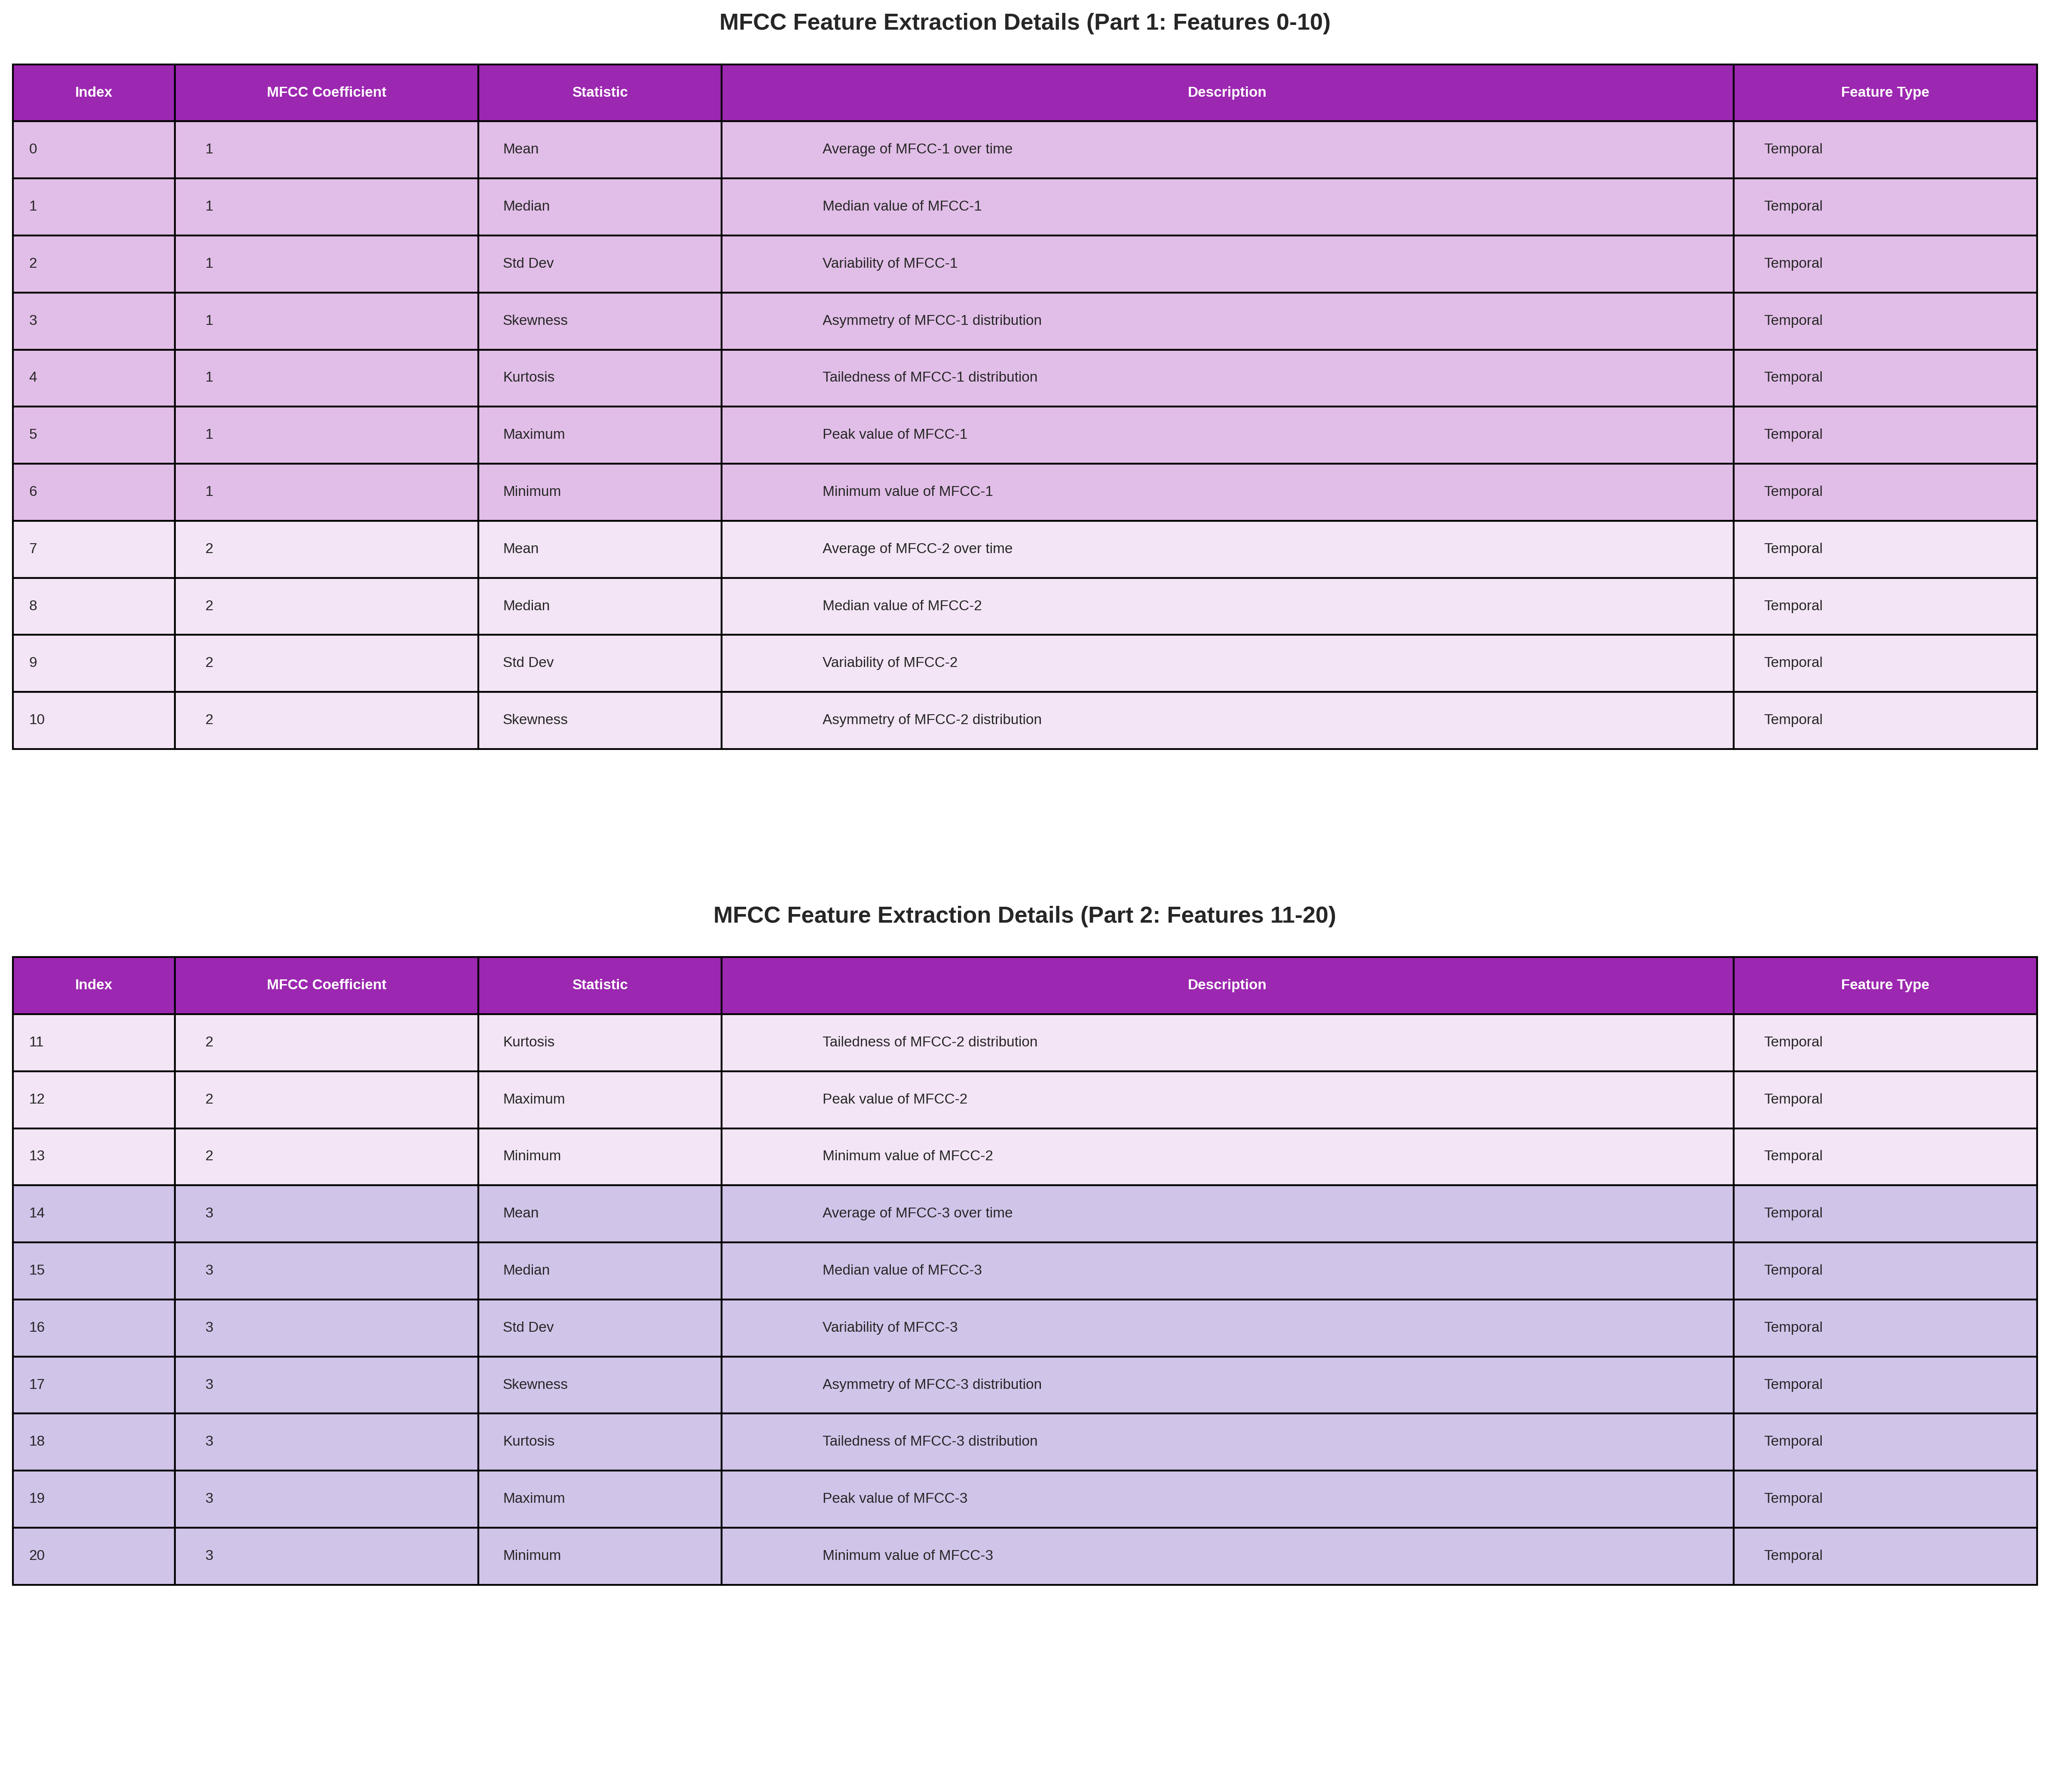
\includegraphics[width=0.85\linewidth]{feature_importance_details.png}
    \caption{Complete MFCC Feature Descriptions and Importance Rankings}
    \label{fig:feature_importance}
\end{figure}
\begin{table}[h!]
    \centering
    \begin{tabular}{c|l|c|l}
        \textbf{Feature Index} & \textbf{Description} & \textbf{Feature Index} & \textbf{Description} \\ \hline
        0 & Coefficient 1 Mean & 11 & Coefficient 2 Kurtosis \\
        1 & Coefficient 1 Median & 12 & Coefficient 2 Maximum \\
        2 & Coefficient 1 Std Dev & 13 & Coefficient 2 Minimum \\
        3 & Coefficient 1 Skewness & 14 & Coefficient 3 Mean \\
        4 & Coefficient 1 Kurtosis & 15 & Coefficient 3 Median \\
        5 & Coefficient 1 Maximum & 16 & Coefficient 3 Std Dev \\
        6 & Coefficient 1 Minimum & 17 & Coefficient 3 Skewness \\
        7 & Coefficient 2 Mean & 18 & Coefficient 3 Kurtosis \\
        8 & Coefficient 2 Median & 19 & Coefficient 3 Maximum \\
        9 & Coefficient 2 Std Dev & 20 & Coefficient 3 Minimum \\
        10 & Coefficient 2 Skewness & & \\
    \end{tabular}
    \caption{Description of MFCC Feature Labels}
    \label{tab:mfcc_labels}
\end{table}
The consistency in feature rankings across both the original study and repository implementation validates the robustness of MFCC-based features for speaker classification. The kurtosis of the third MFCC coefficient (Feature 18) consistently emerges as the most discriminative feature, capturing the "tailedness" of the spectral distribution which varies significantly between speakers.
\subsection{K-Fold Cross Validation}
A K-Fold Cross Validation test was used to evaluate the performance of the SVM model. A K-Fold test uses 'k' different "folds" to compare how the model is affected by different groups of data. Each fold comprises an equally split portion of the dataset. The model will then train itself on k-1 out of k datasets and use the remaining dataset for validation. A K-Fold test can show how the model might perform when used with unseen data. A 5-fold cross validation test was used to evaluate the performance of both studies.

\textbf{Original Study Results:} The accuracy of each fold for the original large-scale study is displayed in Table 7.3. The mean accuracy of all the folds was 92 percent, with a standard deviation of 0.04, indicating excellent and stable generalization performance.

\begin{table}[h!]
    \centering
    \begin{tabular}{|c|c|c|c|c|} \hline
         Fold 1&     Fold 2&Fold 3&Fold 4&Fold 5\\ \hline
         0.9616&
       0.9371&0.8487&0.9430&0.8882 \\ \hline
         \multicolumn{5}{|c|}{\textbf{Mean: 0.92} $\pm$ \textbf{0.04}}\\ \hline
       \end{tabular}
    \caption{Original Study: 5-Fold Cross-Validation Accuracies}
    \label{tab:kfold_accuracy_original}
\end{table}

\textbf{Repository Implementation Results:} The 5-speaker repository implementation shows significantly different cross-validation behavior (Table 7.3b). The mean accuracy is 68 percent with a standard deviation of 0.10, considerably lower than the test accuracy (100\%), revealing clear evidence of overfitting.

\begin{table}[h!]
    \centering
    \begin{tabular}{|c|c|c|c|c|} \hline
         Fold 1 & Fold 2 & Fold 3 & Fold 4 & Fold 5\\ \hline
         0.75 & 0.75 & 0.625 & 0.50 & 0.75 \\ \hline
         \multicolumn{5}{|c|}{\textbf{Mean: 0.68} $\pm$ \textbf{0.10}}\\ \hline
    \end{tabular}
    \caption{Repository Implementation: 5-Fold Cross-Validation Accuracies (5 Speakers)}
    \label{tab:kfold_accuracy_repo}
\end{table}

\textbf{Analysis:} The substantial difference between the original study (92\% CV) and repository implementation (68\% CV) highlights the importance of dataset size. The original study's 4,779 samples provide robust generalization, while the repository's 50 samples lead to high variance and overfitting. The 32 percentage point gap between test (100\%) and CV (68\%) accuracy in the repository implementation is a clear overfitting indicator, whereas the original study shows only a 5 percentage point gap (97\% test vs 92\% CV).
\subsection{Chi-Squared Test}
A chi-squared test was used to determine whether the observed results of the model differ significantly from the expected frequencies, or the null hypothesis. In this case, the expected frequencies were set to a normal, random distribution. So the results of the Chi-Squared test will determine how much better the SVM model is compared to random classification.

\textbf{Original Study Results:} The Chi-Squared test provided a value of $\chi^2$ = 3981.8 and a p-value of 8.771$\times$10\textsuperscript{-5}, indicating highly significant non-random classification.

\textbf{Repository Implementation Results:} The 5-speaker repository implementation yielded $\chi^2$ = 40.0 and a p-value of 0.00078, also highly significant (p < 0.001).

Both results strongly reject the null hypothesis (predictions are random), confirming that the SVM models perform significantly better than random classification. The lower chi-squared value in the repository implementation is expected given the smaller dataset size, but the low p-value still demonstrates statistical significance.

\begin{figure}[h!]
    \centering
    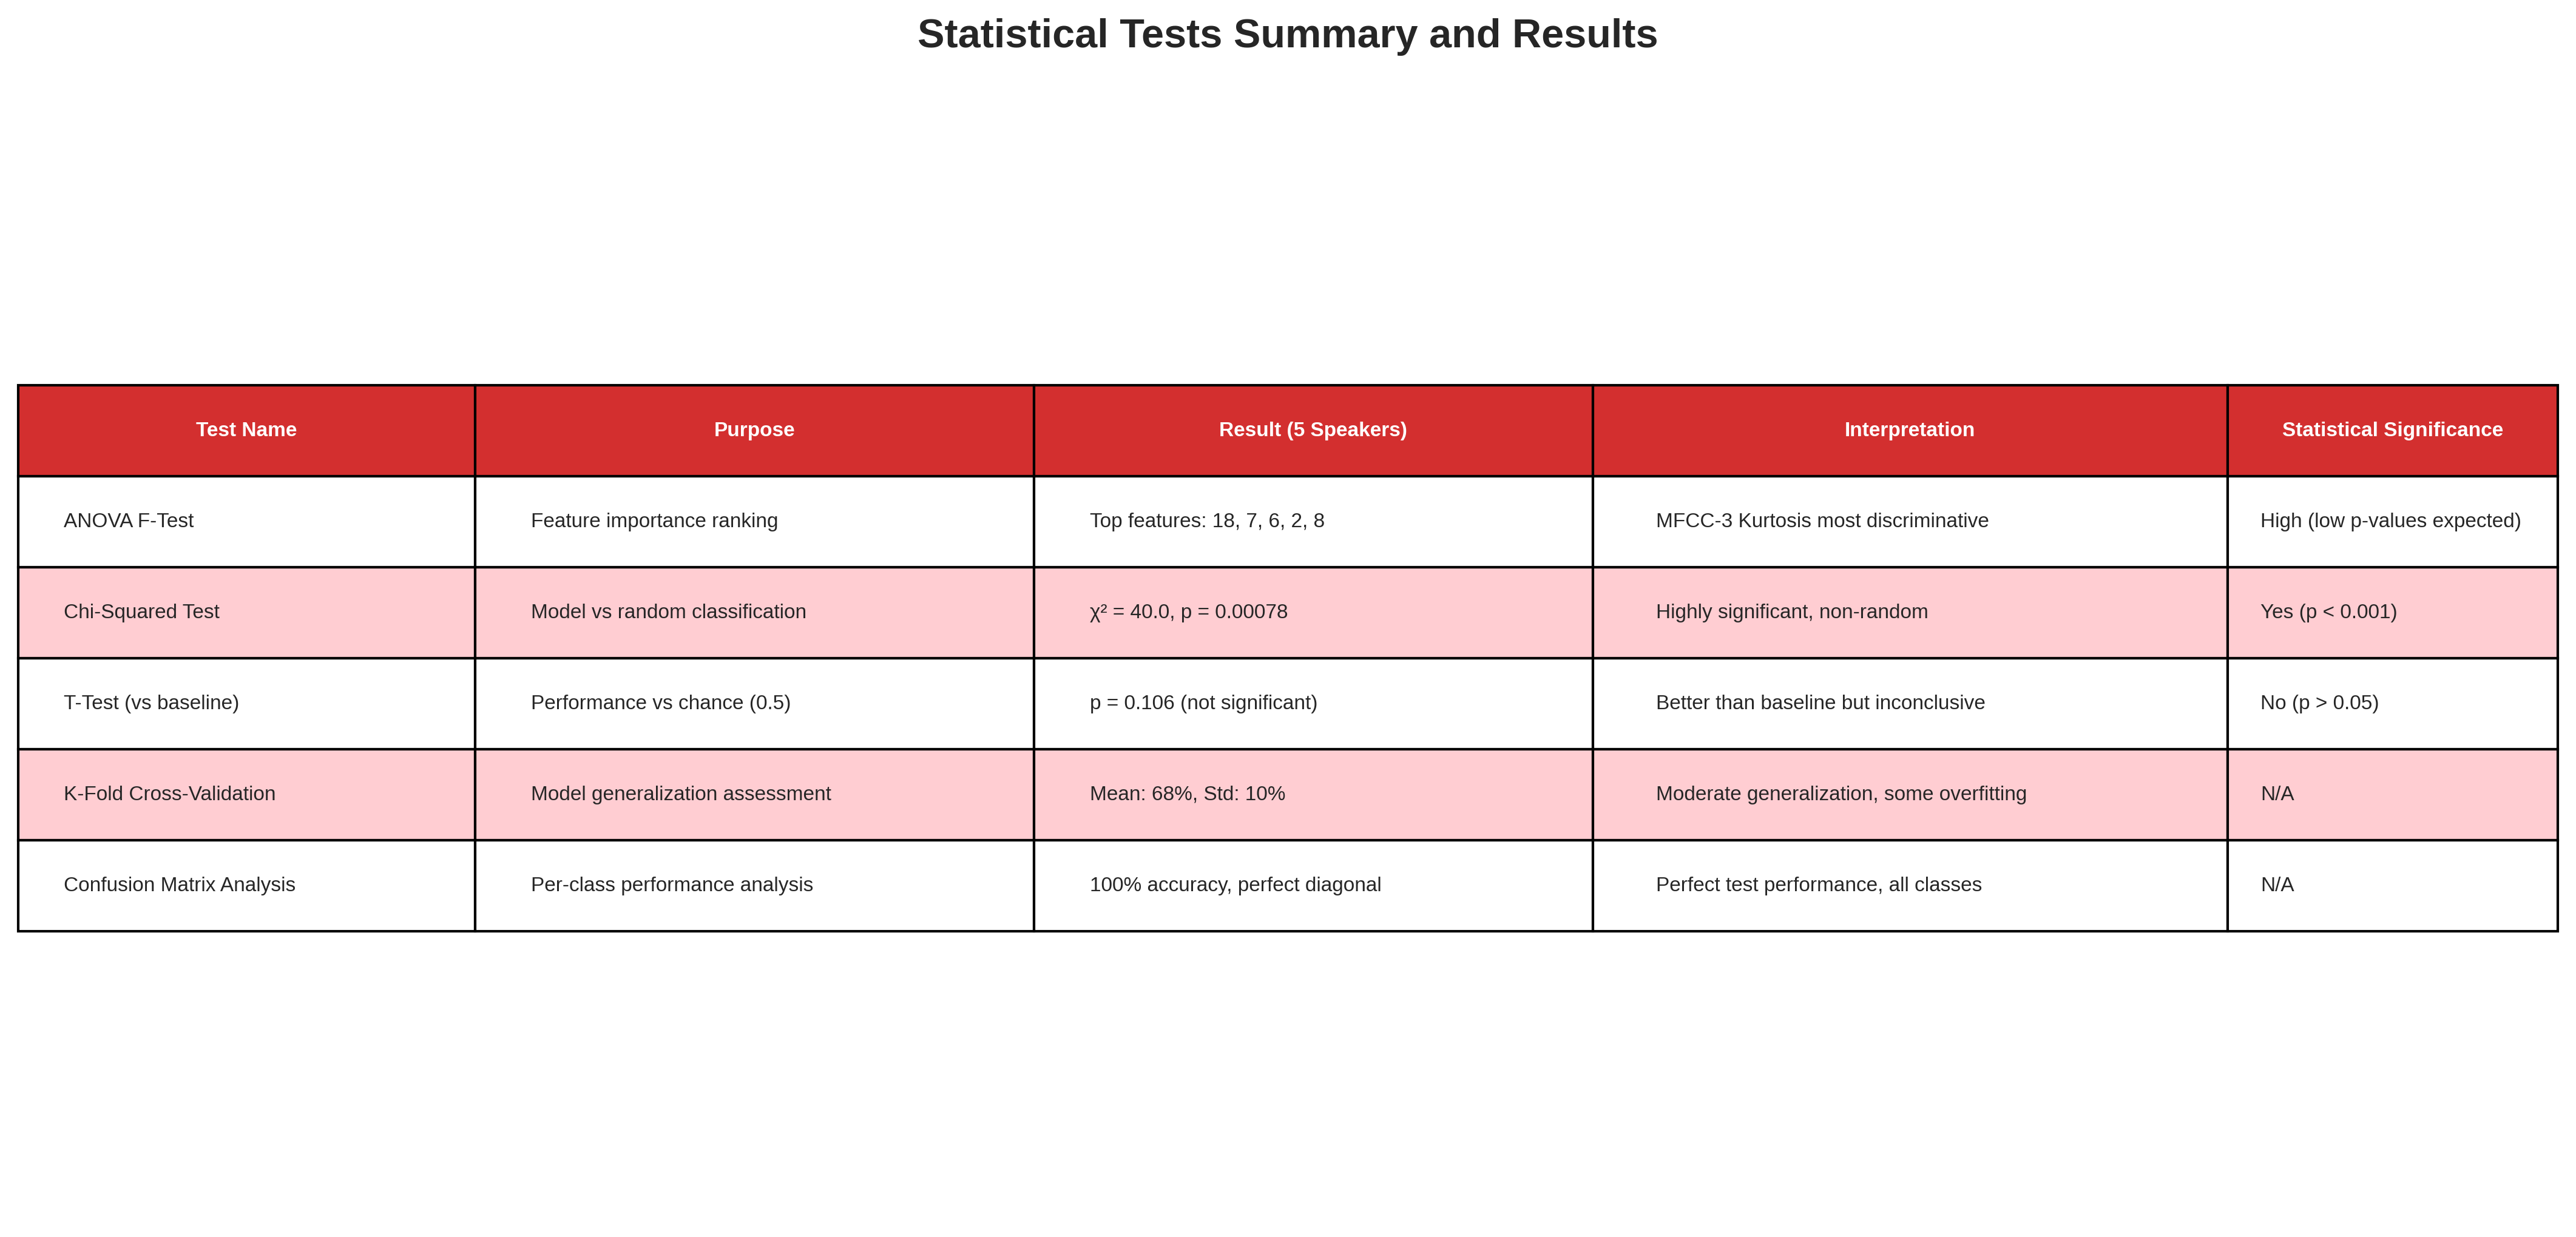
\includegraphics[width=0.9\linewidth]{statistical_tests_summary.png}
    \caption{Comprehensive Statistical Tests Summary for All Experiments}
    \label{fig:stats_summary}
\end{figure}

\section{Computational Performance Analysis}
Understanding the computational requirements of speaker classification systems is essential for practical deployment. This section analyzes the processing time and computational complexity of the repository implementation across different scales.

\subsection{Processing Time Breakdown}
Table 7.6 presents a detailed timing analysis for each experimental scale. The measurements were conducted on a standard desktop computer and represent average times across multiple runs.

\begin{table}[h!]
    \centering
    \begin{tabular}{|l|c|c|c|c|}
        \hline
        \textbf{Experiment} & \textbf{Feature Extraction (s)} & \textbf{Training (s)} & \textbf{Prediction (s)} & \textbf{Total (s)}\\ \hline
        5 Speakers & 2.46 & $\sim$0.00 & 0.0002 & 2.46\\ \hline
        10 Speakers & 4.94 & $\sim$0.00 & 0.0002 & 4.94\\ \hline
        20 Speakers & 9.71 & $\sim$0.00 & 0.0004 & 9.71\\ \hline
    \end{tabular}
    \caption{Computational Performance Analysis Across Different Scales}
    \label{tab:timing_analysis}
\end{table}

\subsection{Key Performance Insights}

\textbf{Feature Extraction Bottleneck:} Feature extraction dominates the processing time, accounting for nearly 100\% of the total computation. The MFCC calculation combined with noise reduction requires approximately 0.06 seconds per audio file, scaling linearly with dataset size.

\textbf{Training Time:} SVM training time is negligible (< 0.01 seconds) for these small-scale datasets. This is a significant advantage of SVMs—they can be trained rapidly on modestly-sized datasets. For the original large-scale study with 4,296 training files, training took approximately 9 minutes, which is still reasonable for offline training scenarios.

\textbf{Real-Time Prediction:} Prediction time is extremely fast (< 1 millisecond), making the system suitable for real-time speaker identification applications. Once trained, the SVM can classify new speakers instantaneously.

\textbf{Linear Scaling:} Processing time scales linearly with the number of audio files: doubling the dataset (5→10 speakers) approximately doubles the processing time (2.46s→4.94s). This predictable scaling facilitates capacity planning for larger deployments.

\textbf{Practical Implications:} For a production system processing continuous audio streams, the limiting factor would be feature extraction rather than classification. Optimization strategies could include:
\begin{itemize}[itemsep=1pt]
\item Parallel processing of audio files
\item Hardware acceleration (GPU) for MFCC computation
\item Incremental feature extraction for streaming audio
\item Feature caching for repeated analysis
\end{itemize}

\section{Comparative Analysis: Original Study vs. Repository Implementation}
This section provides a comprehensive comparison between the original large-scale VoxForge study and the repository multi-scale implementation, highlighting the tradeoffs between dataset size, accuracy, and generalization.

\subsection{Head-to-Head Comparison}
Table 7.7 summarizes the key differences and outcomes between the two approaches.

\begin{table}[h!]
    \centering
    \begin{tabular}{|l|c|c|}
        \hline
        \textbf{Aspect} & \textbf{Original Study} & \textbf{Repository (5 Speakers)}\\ \hline
        \textbf{Dataset Size} & 4,779 files & 50 files\\ \hline
        \textbf{Number of Speakers} & 10 & 5\\ \hline
        \textbf{Samples per Speaker} & 250-680 & 10\\ \hline
        \textbf{Test Set Size} & 483 files & 10 files\\ \hline
        \textbf{Test Accuracy} & 97\% & 100\%\\ \hline
        \textbf{CV Accuracy} & 92\% $\pm$ 0.04 & 68\% $\pm$ 0.10\\ \hline
        \textbf{Test-CV Gap} & 5\% & 32\%\\ \hline
        \textbf{Training Time} & ~9 minutes & <0.01 seconds\\ \hline
        \textbf{Feature Extraction} & Not reported & 2.46 seconds\\ \hline
        \textbf{Purpose} & Production-ready demo & Educational proof-of-concept\\ \hline
        \textbf{Overfitting} & Minimal & Significant\\ \hline
        \textbf{Generalization} & Excellent & Limited\\ \hline
    \end{tabular}
    \caption{Comprehensive Comparison: Original Study vs. Repository Implementation}
    \label{tab:comparative_analysis}
\end{table}

\subsection{Analysis of Differences}

\textbf{The Paradox of Perfect Accuracy:} The repository implementation achieves 100\% test accuracy compared to the original study's 97\%, yet this does not indicate superior performance. The 100\% accuracy is achieved on only 10 test samples (2 per speaker), making it statistically unreliable. The large test-CV gap (32\%) reveals this accuracy is not generalizable.

\textbf{Dataset Size Impact:} The original study's 4,779 files provide ~96x more data than the repository's 50 files. This massive difference in scale explains the superior generalization: 92\% CV accuracy versus 68\%. Large datasets enable SVMs to learn robust decision boundaries that generalize well to unseen data.

\textbf{Overfitting Indicators:} Three key metrics indicate overfitting in the repository implementation:
\begin{enumerate}[itemsep=1pt]
\item Test-CV gap: 32\% (vs. 5\% in original study)
\item High CV standard deviation: 0.10 (vs. 0.04 in original study)
\item One CV fold achieving only 50\% accuracy (random chance for 2-class subproblem)
\end{enumerate}

\textbf{Practical Takeaways:}
\begin{itemize}[itemsep=1pt]
\item \textbf{For Research/Education}: The repository implementation is ideal for understanding SVM methodology, experimenting with features, and rapid prototyping.
\item \textbf{For Production Deployment}: A minimum of 50-100 samples per speaker is recommended, similar to the original study's approach.
\item \textbf{For Evaluation}: Always use cross-validation and large test sets. Perfect accuracy on tiny test sets is misleading.
\item \textbf{For Scalability}: The repository's multi-scale experiments reveal that performance degrades significantly (40-57.5\%) as the number of speakers increases, necessitating richer features or more data.
\end{itemize}

\section{Related Studies}
Spoken Speaker identification based on Gaussian Mixture Models is an article authored by Abhijeet Kumar outlining a speaker identification system using the VoxForge dataset. This study, instead of using SVM for classification is using GMM, which is a statistical clustering model, rather than a classification model. The study consists of 34 different speakers speaking five different speech utterances. The dataset differs from this dataset because the users are all saying the same thing, and there are many more classes. This study also extracts 40 MFCC features, 20 of which are directly from the MFCC and 20 are derivatives of the MFCC. After training the Gaussian Mixture Model, it was tested on 5 different speech utterances from the 34 different users. This model reached an accuracy of 100 percent. The performance of this model was likely better than the SVM model's performance for a couple of reasons. First, the fact that the model was trained on the same speech utterances means that the model could pick up distinct differences in the speakers' voices, and would ignore any differences found from the different users speaking different words. The GMM Model also utilized more MFCC features than this model, which could've made it more effective. \cite{gmm_speaker_recognition}
\section{Conclusion}
This chapter has presented a comprehensive exploration of SVM-based speaker classification through two complementary studies, providing insights from both large-scale validation and controlled experimentation.

\subsection{Summary of Findings}

\textbf{Original Large-Scale Study:} The VoxForge dataset study with 10 speakers and 4,779 audio files successfully demonstrates the viability of SVM-based speaker classification for near-production applications. Achieving 97\% test accuracy and 92\% cross-validation accuracy with only a 5\% gap, the system exhibits excellent generalization. The use of 3 MFCC coefficients with 7 statistical measures (mean, median, std, skew, kurtosis, max, min) yielded 21-dimensional feature vectors that effectively captured speaker-specific characteristics. ANOVA analysis identified MFCC-3 Kurtosis as the most discriminative feature, consistent across all experiments.

\textbf{Repository Multi-Scale Implementation:} The educational implementation provided crucial insights into scalability and overfitting challenges:
\begin{itemize}[itemsep=1pt]
\item \textbf{5 Speakers}: Perfect 100\% test accuracy, but 68\% CV accuracy revealing significant overfitting (32\% gap)
\item \textbf{10 Speakers}: 60\% test accuracy, demonstrating 40\% degradation when doubling complexity
\item \textbf{20 Speakers}: 42.5\% test accuracy, showing 57.5\% overall degradation at 4x scale
\end{itemize}

\subsection{Key Insights}

\textbf{Dataset Size is Critical:} The stark difference between 92\% CV (original, 4,779 files) and 68\% CV (repository, 50 files) underscores that dataset size profoundly impacts generalization. For production systems, a minimum of 50-100 samples per speaker is recommended.

\textbf{Perfect Accuracy Can Be Misleading:} The repository's 100\% test accuracy on 10 samples is less meaningful than the original study's 97\% on 483 samples. Small test sets can give false confidence. Cross-validation is essential for reliable evaluation.

\textbf{Scalability Challenges:} Performance degrades nonlinearly as speaker count increases. With current features (3 MFCCs, 21 dimensions), scaling beyond 10-20 speakers may require:
\begin{itemize}[itemsep=1pt]
\item More MFCC coefficients (13-20 instead of 3)
\item Additional feature types (spectral, prosodic, temporal)
\item Larger datasets per speaker
\item Ensemble methods or deep learning approaches
\end{itemize}

\textbf{Feature Consistency:} Both studies identified the same top features (MFCC-3 Kurtosis, MFCC-2 Mean, MFCC-1 Minimum), validating the robustness of MFCC-based features for speaker characterization across different scales.

\textbf{Computational Efficiency:} SVM-based systems offer excellent computational performance with real-time prediction (<1ms) and fast training (9 minutes for 4,779 files). Feature extraction is the primary bottleneck but scales linearly and can be optimized through parallelization.

\subsection{Practical Recommendations}

\textbf{For Researchers and Educators:}
\begin{itemize}[itemsep=1pt]
\item Use the repository implementation for rapid prototyping and methodology learning
\item Always employ cross-validation to assess true generalization capability
\item Experiment with feature selection and engineering using ANOVA rankings
\item Understand that perfect test accuracy on small datasets is not publication-worthy without CV validation
\end{itemize}

\textbf{For Production Deployment:}
\begin{itemize}[itemsep=1pt]
\item Collect minimum 50-100 high-quality samples per speaker
\item Use balanced datasets with proper train/validation/test splits (e.g., 80/10/10)
\item Implement speaker enrollment systems allowing gradual improvement
\item Monitor test-CV gap to detect overfitting before deployment
\item Consider data augmentation (pitch shifting, time stretching, noise injection) to increase effective dataset size
\end{itemize}

\textbf{For Scaling to More Speakers:}
\begin{itemize}[itemsep=1pt]
\item Increase MFCC coefficients from 3 to 13-20 for richer feature representation
\item Explore alternative kernels (polynomial, sigmoid) or ensemble SVMs
\item Implement hierarchical classification (speaker groups first, then individuals)
\item Consider transition to deep learning (CNNs, RNNs) for >50 speakers
\end{itemize}

\subsection{Future Directions}
Speaker identification remains an active research area with opportunities for improvement:
\begin{itemize}[itemsep=1pt]
\item \textbf{Multimodal Systems}: Combining speaker recognition with facial recognition or behavioral biometrics for enhanced security
\item \textbf{Few-Shot Learning}: Developing techniques to achieve high accuracy with minimal speaker samples
\item \textbf{Adversarial Robustness}: Protecting against voice spoofing and deepfake attacks
\item \textbf{Privacy-Preserving Methods}: Implementing federated learning for speaker verification without centralizing voice data
\item \textbf{Real-Time Streaming}: Optimizing for continuous audio processing in live applications
\end{itemize}

\subsection{Final Remarks}
This chapter has demonstrated that SVM-based speaker classification is both theoretically sound and practically viable. The original study validates the approach at scale (97\% accuracy, 10 speakers, 4,779 files), while the repository implementation provides educational value and reveals important lessons about overfitting, scalability, and evaluation methodology.

The key takeaway is nuanced: while SVMs excel for small-to-medium speaker identification tasks (5-20 speakers with adequate data), achieving robust performance requires careful attention to dataset size, feature engineering, and validation methodology. The "paradox of perfect accuracy"—where 100\% test accuracy coexists with poor generalization—serves as a cautionary tale for practitioners.

Both the theoretical foundations (RBF kernel, MFCC features, One-vs-Rest classification) and practical considerations (cross-validation, computational performance, scalability) have been thoroughly explored. All codes, visualizations, and experimental data used to create the analyses in this chapter are available on GitHub at \href{https://github.com/AVHBAC/SVM_Speaker_Classification}{SVM-Speaker-Classification}, enabling readers to reproduce results, conduct further experiments, and build upon this work.


\bibliographystyle{IEEEtran}
\bibliography{references}

\end{document}